\section{Dataset Construction}

\subsection{Data Collection and Sources}

We construct a high-quality, multi-source balanced circuit schematic OCR dataset~\citep{zhang2026circuitocrfinal}, comprising three sources:

\textbf{Source 1: Programmatic Synthetic Renderings (Synthetic V3, 500 images).} 500 circuit schematic images are randomly generated via Python scripts~\citep{zhang2026circuitocr}. The generation pipeline: the program randomly generates circuit topology specifications (5--30 components with mixed connections), automatically draws schematic symbols (10 component types: resistors, capacitors, inductors, diodes, LEDs, transistors, ICs, connectors, crystals, fuses), and renders them as PNG images. \textbf{Ground truth labels are directly derived from \texttt{draw.text()} call logs}---every text write operation records its content and position synchronously; labels are generated by sorting all recorded text in spatial reading order (top-to-bottom, left-to-right). This mechanism ensures 100\% alignment between GT and visible on-image text, fundamentally eliminating annotation bias.

\textbf{Source 2: Real-World KiCad Open-Source Schematics (train-real, 1,357 images).} Collected from the GitHub/KiCad open-source hardware community under CC-BY-4.0 and similar open-source licenses. Images are rendered via kicad-cli SVG export $\to$ cairosvg PNG at high quality. GT labels are extracted from SVG stroked-text visible text elements and arranged in a one-word-per-line vertical format (98.6\% consistent with the test set format). Labels cover component reference designators (R1, C5, U3), parameter values (10k, 100$\mu$F, STM32F103), and net labels (VCC, GND, +5V), strictly excluding invisible KiCad internal symbols and hidden-layer text.

\textbf{Source 3: Masala-CHAI Textbook Circuit Diagrams (698 images, filtered).} From the Masala-CHAI open-source dataset~\citep{bhandari2025masalachai} under CC-BY-4.0. The original dataset contains approximately 7,500 textbook circuit diagrams with accompanying SPICE netlists. We extract component reference designators (e.g., R1, M1, Q2) and types/parameter values (e.g., NMOS, 10k, NPN) from the SPICE netlists to generate concise OCR-format labels. Out of 4,858 initially valid samples, we apply SPICE artifact cleaning (removing 437 samples containing formula expressions, simulation directives, and placeholder templates), quality scoring (composite score based on line count, character diversity, and component type variety), and stratified sampling to select 698 high-quality samples, forming a 0.38:1 ratio against the KiCad data.

\subsection{Data Filtering and Quality Control}

The V5 Golden dataset's quality control is guided by four core principles:

\textbf{Principle 1: GT must fully align with visible on-image text.} Earlier dataset versions (V1--V2) generated GT labels from the KiCad data model (S-expression parsing), which included large amounts of text invisible on rendered images---pin numbers, hidden net names, etc.---severely corrupting the training signal. V5 fundamentally changes this strategy: synthetic data uses draw.text() synchronous recording; real KiCad data extracts visible text from SVG stroked-text elements; Masala-CHAI extracts component information from SPICE netlists (not OCR).

\textbf{Principle 2: Multi-source balance prevents distribution bias.} Using all 4,858 Masala-CHAI samples would make them 85.5\% of the training set, causing the model to be dominated by SPICE format at the expense of KiCad schematic literal OCR capability. We downsample Masala-CHAI to 698, forming a 0.38:1 ratio against 1,857 KiCad samples, ensuring the model treats KiCad vertical format as primary and Masala SPICE format as supplementary.

\textbf{Principle 3: No AI labeling AI.} All GT labels come from deterministic rules (program logging, SPICE parsing, SVG element extraction). No OCR model or other AI system is ever used to generate annotations, ensuring absolute GT authenticity and reproducibility.

\textbf{Principle 4: Format alignment with the test set.} We discovered that the Open Schematics and Rescraped subsets in the V4 dataset exhibited severe format mismatch (horizontal space-concatenated format vs.\ the test set's one-word-per-line vertical format) and duplication noise (22,340 intra-line adjacent duplicate word pairs). V5 completely removes these two noise sources. The train-real label format (97.9\% single-word lines) is nearly perfectly aligned with the test set (98.6\% single-word lines), and intra-line duplication noise dropped from 22,340 to 107 (99.5\% reduction).

\paragraph{Masala-CHAI SPICE Cleaning Pipeline}

Masala-CHAI raw SPICE netlists contain four categories of artifacts requiring cleaning:
\begin{enumerate}[nosep]
    \item \textbf{SPICE comments and directives:} Comment lines beginning with semicolon (;) or asterisk (*), simulation control directives (.tran, .ac, .dc, .op, etc.);
    \item \textbf{Mathematical formula expressions:} Brace-enclosed expressions (e.g., \texttt{\{gm*v(4,8)\}}), VALUE= assignment statements;
    \item \textbf{Device dimension parameters:} MOSFET L=/W= parameters (e.g., \texttt{L=40n W=300u}), SPICE node names (e.g., \texttt{net7}, \texttt{net23});
    \item \textbf{Placeholder templates:} Angle-bracket or square-bracket enclosed placeholder values (e.g., \texttt{<Voltage\_Value>}, \texttt{[value]}).
\end{enumerate}
After cleaning, 4,858 $\to$ 4,421 clean samples remain. We then apply composite quality scoring based on three metrics: line count (preferring 5--15 line rich samples), character diversity, and component type variety. The top 60\% by score are selected, with the remaining 40\% drawn via stratified sampling across line-count buckets to ensure long-tail coverage, yielding 698 high-quality samples.

\subsection{Dataset Split and Statistics}

After the above cleaning and filtering, the final dataset contains \textbf{2,555 independent schematic samples}, split 90\%/10\% into training and validation sets: 2,299 training samples and 256 validation samples. The test set reuses the existing 523-sample benchmark (easy50/100/200/full523) to maintain comparability with prior experiments. Table~\ref{tab:dataset} lists key statistics for each data source.

\begin{table}[h]
\centering
\caption{Dataset Composition and Source Statistics (V5 Golden)}
\label{tab:dataset}
\begin{tabular}{lcccl}
\toprule
\textbf{Source} & \textbf{Count} & \textbf{License} & \textbf{GT Generation Method} & \textbf{GT Quality} \\
\midrule
Synthetic V3      & 500   & Apache 2.0 & draw.text() sync recording  & 100\% aligned \\
train-real (KiCad)& 1,357 & CC-BY-4.0  & SVG stroked-text extraction & Visible text \\
Masala-CHAI       & 698   & CC-BY-4.0  & SPICE netlist + cleaning    & Deterministic \\
\midrule
\textbf{KiCad subtotal}& \textbf{1,857} & -- & -- & -- \\
\textbf{Masala subtotal}& \textbf{698} & -- & 0.38:1 ratio vs.\ KiCad & -- \\
\midrule
\textbf{Total}     & \textbf{2,555} & -- & Analog/Digital/Mixed-signal/Power & -- \\
\bottomrule
\end{tabular}
\par\smallskip
{\small\noindent Note: (1) Masala-CHAI raw 4,858 samples were cleaned of SPICE artifacts (437 removed), quality-scored, and stratified-sampled to select 698.\\
(2) Compared to V4, V5 removes the Open Schematics (226) and Rescraped (102) subsets which exhibited format mismatch and duplication noise.}
\end{table}

\begin{figure}[h]
\centering
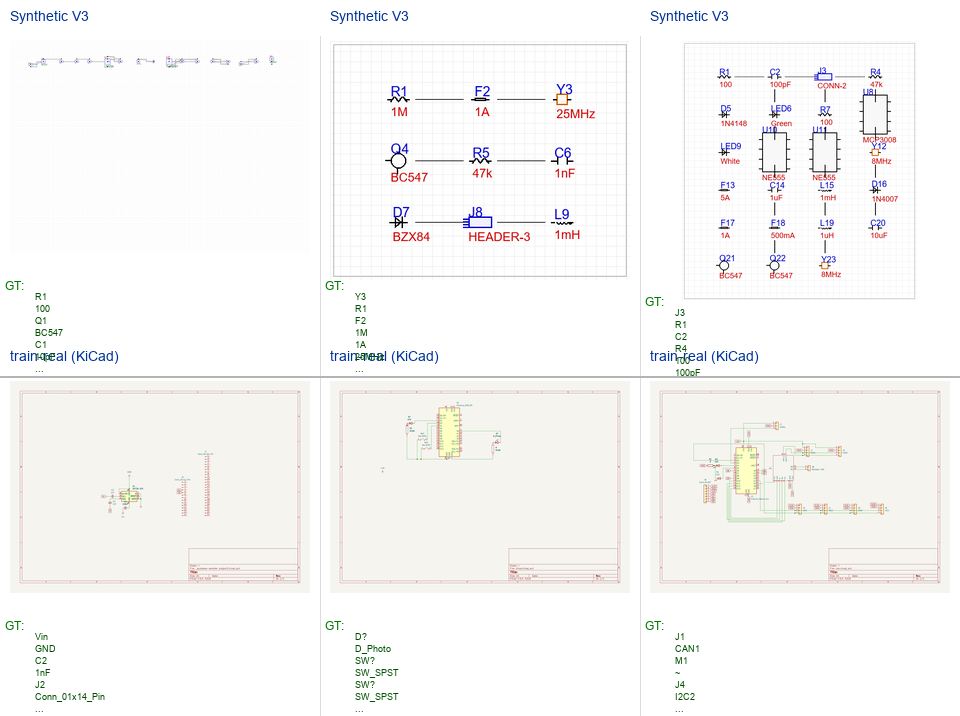
\includegraphics[width=\textwidth]{../circuit-ocr-dataset/figures/dataset_samples.png}
\caption{V5 Golden dataset samples. Three rows respectively from Synthetic V3, train-real, and Masala-CHAI, demonstrating dataset diversity coverage: from programmatically generated simple schematics to complex real-world open-source PCB designs, from textbook SPICE-style labels to one-word-per-line KiCad vertical format.}
\label{fig:dataset_samples}
\end{figure}

\begin{figure}[h]
\centering
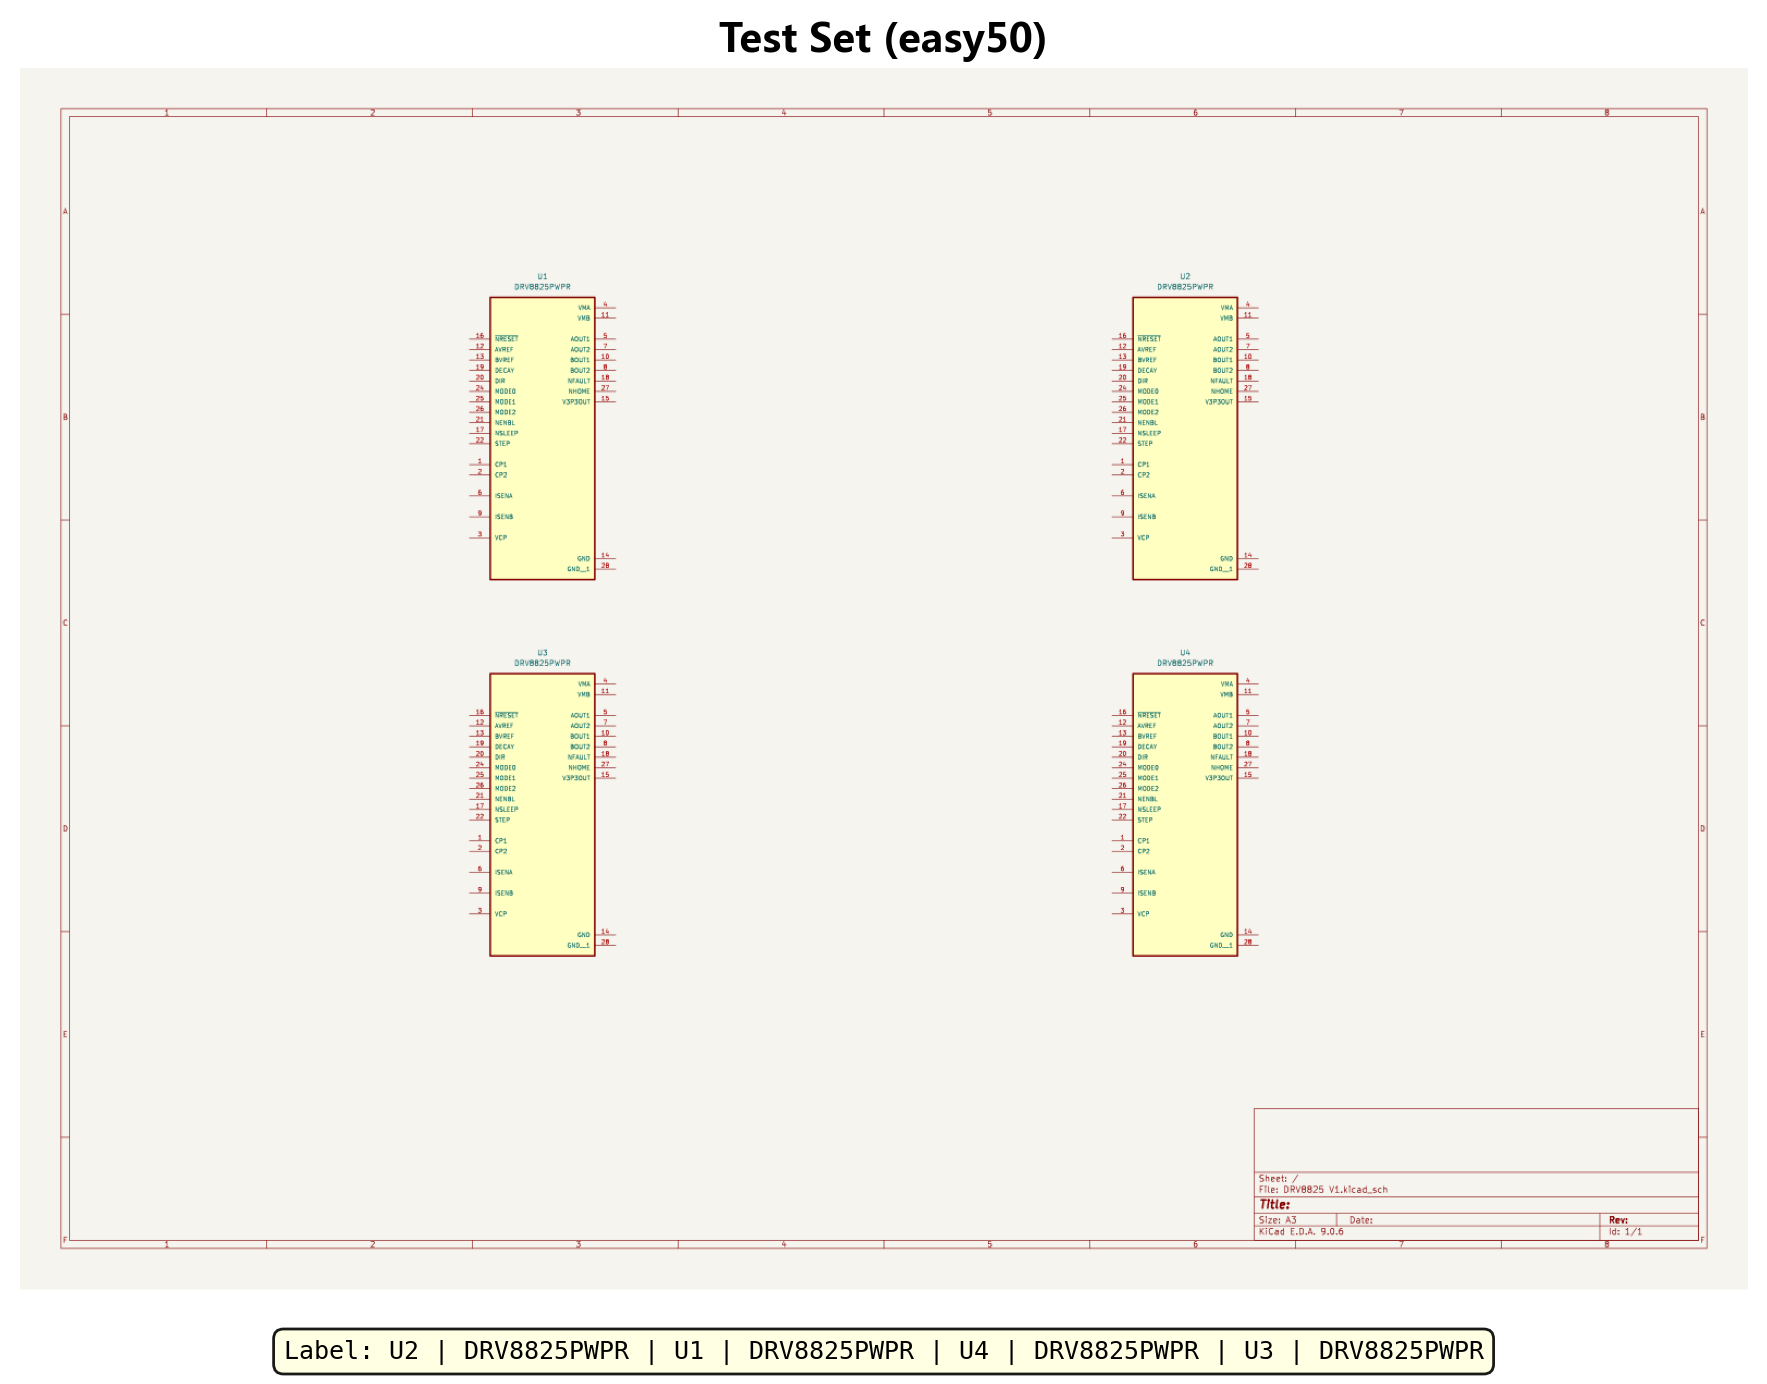
\includegraphics[width=\textwidth]{../circuit-ocr-dataset/figures/dataset_Test_Set.png}
\caption{Test set samples. 523 test samples divided into four difficulty tiers by annotation length: easy50 (27--109 chars), easy100 (27--163 chars), easy200 (27--296 chars), and full523 (all 523 samples), enabling systematic model capability assessment.}
\label{fig:dataset_test}
\end{figure}

\subsection{Dataset Split Details}

Table~\ref{tab:split} shows detailed statistics for each split tier.

\begin{table}[h]
\centering
\caption{Training/Validation/Test Split Statistics}
\label{tab:split}
\begin{tabular}{lcccccc}
\toprule
\textbf{Split} & \textbf{Samples} & \textbf{KiCad} & \textbf{Masala} & \textbf{avg Lines} & \textbf{med Lines} & \textbf{avg Chars} \\
\midrule
Training   & 2,299 & 1,666 & 633 & 34.4 & 33 & 286 \\
Validation & 256   & 191  & 65  & 35.6 & 34 & 304 \\
Test       & 523   & 523  & 0   & -- & -- & -- \\
\midrule
\textbf{Total} & \textbf{3,078} & 2,380 & 698 & -- & -- & -- \\
\bottomrule
\end{tabular}
\par\smallskip
{\small\noindent Note: The test set comes from the existing benchmark (easy50/100/200 + full523), all from KiCad sources, with zero overlap with training/validation sets.}
\end{table}

\textbf{Label Format Characteristics.} KiCad-source labels follow a one-word-per-line vertical format (e.g., \texttt{R1\textbackslash n10k\textbackslash nGND}), consistent with the schematic's spatial reading order and 98.6\% aligned with the test set format. Masala-CHAI-source labels follow a SPICE netlist style---one component per line (e.g., \texttt{R1 10k}), compact and concise (median 4 lines, 48 characters). Mixed-format training enables the model to simultaneously learn literal OCR (KiCad vertical format) and structured netlist output (Masala horizontal format). During evaluation, the \texttt{--unordered} flag sorts predicted and reference lines alphabetically before computing NED, eliminating reading-order and format differences from affecting evaluation.

\textbf{Circuit Type Coverage.} The dataset covers four major circuit categories: analog circuits (op-amps, filters, power management), digital circuits (logic gates, MCU peripherals, memory interfaces), mixed-signal circuits (ADC/DAC, PLL), and power circuits (DC-DC converters, LDO regulators). Programmatic generation of the synthetic dataset ensures sufficient training samples for each type, while Masala-CHAI's textbook origin supplements classical circuit topologies from educational scenarios.

\subsection{Data Augmentation Strategy}
During training, we apply the following online augmentations to each input image: random JPEG compression (quality factor 85--100), random scaling (max dimension 168--384 pixels), and random horizontal flipping. These lightweight augmentations simulate real-world image quality variations while preserving circuit schematic readability.

